A biological neural network (brain) consists of cells called neurons. Human brain is composed of about 10 billion neurons, each connected to about 10,000 other neurons. The same applies to artificial neural network - they consists of many artificial neurons - mathematical models of biological ones. I will start this section by describing the structure of a biological neuron. Then I will provide a formal description of an artificial neuron as a mathematical model.

\paragraph{Biological neurons} According to the medical definition, provided by Merriam-Webster dictionary\footnote{http://www.merriam-webster.com/dictionary/neuron},
\begin{quote}
  Neuron is a cell that carries messages between the brain and other parts of the body and that is the basic unit of the nervous system.
\end{quote}

Figure \ref{fig:bioneuron} shows the simplified schematic of a biological neuron. Each neuron consists of a cell body, or soma, that contains a cell nucleus. Branching out from the cell body are a number of fibers called dendrites and a single long fiber called the axon. The axon stretches out for a long distance, much longer than the scale in this diagram indicates. Typically, an axon is 1 cm long (100 times the diameter of the cell body), but can reach up to 1 meter. A neuron makes connections with 10 to 100,000 other neurons at junctions called synapses. Signals are propagated from neuron to neuron by a complicated electrochemical reaction. The signals control brain activity in the short term and also enable long-term changes in the connectivity of neurons. These mechanisms are thought to form the basis fur learning in the brain.
Each neuron receives electrochemical inputs from other neurons at the dendrites.  If the sum of these electrical inputs is sufficiently powerful to activate the neuron, it transmits an electrochemical signal along the axon, and passes this signal to the other neurons whose dendrites are attached at any of the axon terminals.
It is important to note that a neuron fires only if the total signal received at the cell body exceeds a certain level.  The neuron either fires or it doesn't, there aren't different grades of firing. 

\begin{figure}[H]
  \centering
  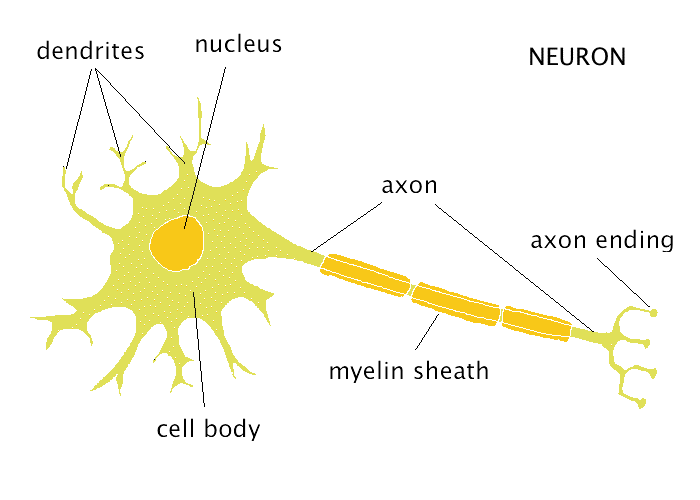
\includegraphics[width=\imgwidth]{bio_neuron}
  \caption{A schematic of biological neuron}
  \label{fig:bioneuron}
\end{figure}

\paragraph{Artificial neurons} 

In fact, artificial neuron can be viewed as a parametric function of $ n $ inputs $ g_{w}:X^{n} \rightarrow Y $, where X is the space of all possible input values, Y - the space of output values and w - the vector of numeric weights $ w_{1}, w_{2}, ..., w_{n} $, the tunable parameters that [...]. In other words, function $ g_{w} $ is [defined with the rule]

\begin{equation}
  y = g_{w}(x)
\end{equation}

where $ x \in X^{n} $, $ y \in Y $ and $ w \in \mathbb{R}^{n} $.

Function $ g_{w} $ is a superposition of two functions, $ s_{w}:X^{n} \rightarrow \mathbb{R} $ and $ f:\mathbb{R} \rightarrow Y $:
\[ g_{w}(x) = f(s_{w}(x)) \]

where $ s_{w} $ is defined as follows:
\[ s_{w}(x) = \sum_{i=0}^{n} w_{i}x_{i} \]

$ f $ is a nonlinear activation function in case of classification and an identity function $ \forall x f(x) = x $ in case of regression.

\begin{figure}[H]
  \centering
  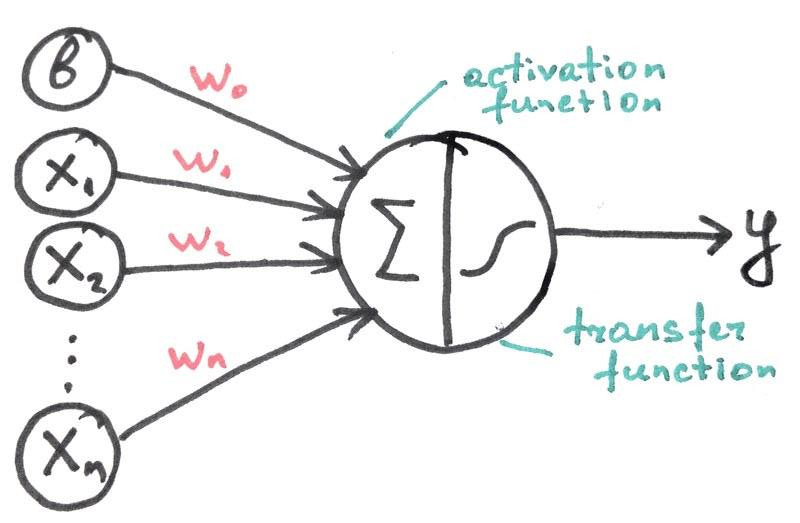
\includegraphics[width=0.8\imgwidth]{artif_neuron}
  \caption[Model of an artifitial neuron]{Model of an artifitial neuron\footnotemark}
  \label{fig:artifneuron}
\end{figure}

\footnotetext{Source: \url{http://www.theprojectspot.com/tutorial-post/introduction-to-artificial-neural-networks-part-1/7}}

%[By type of activation function neurons are divided ...
%Hard and soft thresholds
%
%Neurons with  hard thresholds are called \textbf{perceptrons}.
